\documentclass[10pt,english]{beamer}
%\documentclass[english,handout]{beamer} % For handouts
\usetheme[progressbar=frametitle,block=fill]{metropolis} %numbering=none

%%% USEFUL PACKAGES
%\usepackage{showframe} % For debugging positioning
\usepackage{etex} % If too many packages
% Encoding and language
\usepackage[utf8]{inputenc}
\usepackage{babel}
\usepackage{amsmath, amssymb}
\usepackage{natbib}
%\usepackage{booktabs}
%\usepackage{algorithmic}
\usepackage{algorithm}
\usepackage{caption}
%\usepackage{animate} % Animations
\usepackage{bm} % Bold math
\usepackage{bbm}
%\usepackage{url}
%\usepackage{pifont}
%\usepackage{ulem} % Used for strikeouts \sout
%\usepackage{stackengine}
%\usepackage{enumitem}
%\setlist[description]{leftmargin=\parindent,labelindent=\parindent}
%\usepackage{colortbl} % Used for colored rows in tables


%%% GRAPHICS
\usepackage{graphicx}
\graphicspath{{./figs/}}


%%% COLORS
\setbeamercolor{background canvas}{bg=white}
\def\BlankFrame{
	\bgroup
	%\pdfpageheight 29.7cm
	\setbeamercolor{background canvas}{bg=}
	\begin{frame}[plain]
	\end{frame}
	%\makeatletter
	%\pdfpageheight \beamer@paperheight
	%\makeatother
	\egroup}

\usepackage{xcolor}
\definecolor{DarkGreen}{HTML}{00B200}
\definecolor{LightBlue}{HTML}{0090D9}
\definecolor{gold}{rgb}{.812,.710,.231}
% Text markup
%\setbeamercolor{alerted text}{fg=red}
\newcommand{\blue}[1]{\textcolor{blue}{#1}}
\newcommand{\red}[1]{\textcolor{red}{#1}}
\newcommand{\grey}[1]{\textcolor{gray}{#1}}
\newcommand{\orange}[1]{\textcolor{mLightBrown}{#1}}
\newcommand\myheading[1]{\textbf{#1}}
\newcommand\myemph[1]{\underline{\emph{#1}}}
\newcommand\textexample[1]{\textit{\textbf{#1}}}

%%% SPACING
\newcommand\vws[1][1]{\vspace{#1\baselineskip}} % vertical white space
%\newcommand\strt[1][1.5ex]{\rule[-.05\baselineskip]{0pt}{#1}} % strut
\newcommand\strt[2]{\rule[-#1ex]{0pt}{#2ex}} % strut
\newcommand\Hrule{\vspace{1ex} \hrule \vspace{1ex}} % Horisontal rule with some space after

%%% MISC
\newcommand\articleref[4]{\noindent\begin{minipage}[t]{0.04\textwidth}
		\vspace{0pt} 
		\pgfuseimage{beamericonarticle}
	\end{minipage}%
	\begin{minipage}[t]{0.96\textwidth}
		\vspace{0pt}
		#1. \textbf{#2.} \textit{#3}, #4.
	\end{minipage}}

%%% METROPOLIS THEME SPECIFIC
\makeatletter
\setlength{\metropolis@progressonsectionpage@linewidth}{1pt}
\makeatother
%\setbeamercolor{progress bar}{fg=red,bg=red!50}


%%% TEXTPOS
\usepackage[absolute,overlay]{textpos} % option showboxes is useful in draft mode
\setlength{\TPHorizModule}{\paperwidth}
\setlength{\TPVertModule}{\paperheight}
\textblockorigin{0pt}{10mm} % start everything at top-left, below gray 


%%% TIKZ/PGFPLOTS
\usepackage{tikz}
\usetikzlibrary{arrows,positioning,calc,shapes.geometric}
%\usetikzlibrary{arrows,calc,shapes.geometric,decorations.pathmorphing,backgrounds,positioning,fit,petri,decorations.pathreplacing}
%\usepackage{pgfplots}
%\pgfplotsset{compat = 1.3}


%%% BLOCKS AND BOXES
% Changing colors of blocks
%\setbeamercolor{block title alerted}{bg=UURed,fg=palette primary.fg}
%\setbeamercolor{block body alerted}{bg=UURed!15}
\setbeamercolor{block title alerted}{bg=mLightBrown,fg=palette primary.fg}
\setbeamercolor{block body alerted}{bg=mLightBrown!15}
%\setbeamercolor{block title example}{bg=UUGreen,fg=palette primary.fg}
%\setbeamercolor{block body example}{bg=UUGreen!10}
% \mybox is a rectangular box
\usepackage{boxedminipage}
\setlength\fboxrule{2pt}
\setlength\fboxsep{2\fboxsep}
\newcommand\mybox[3][\textwidth]{
  {\color{#2}
    \begin{boxedminipage}{#1}
      {\color{palette primary.bg} #3}
    \end{boxedminipage}}%
}   
\usepackage{tcolorbox}
\tcbset{arc=1mm,grow to left by=3mm,grow to right by=3mm,left=2mm}
%\newenvironment{redbox}{%
%	\begin{tcolorbox}[colback=UURed!15,colframe=UURed]}{%
%	\end{tcolorbox}}
%\newenvironment{greenbox}{%
%	\begin{tcolorbox}[colback=UUGreen!15,colframe=UUGreen]}{%
%	\end{tcolorbox}}
\newenvironment{redbox}{%
	\begin{tcolorbox}[colback=red!15,colframe=red]}{%
	\end{tcolorbox}}
\newenvironment{greenbox}{%
	\begin{tcolorbox}[colback=DarkGreen!15,colframe=DarkGreen]}{%
	\end{tcolorbox}}
\newenvironment{graybox}{%
	\begin{tcolorbox}[colback=mDarkTeal!5,colframe=mDarkTeal]}{%
	\end{tcolorbox}}
\newenvironment{orangebox}{%
\begin{tcolorbox}[colback=mLightBrown!15,colframe=mLightBrown]}{%
	\end{tcolorbox}}
\newenvironment{bwbox}{%
	\begin{tcolorbox}[colback=white,colframe=black]}{%
\end{tcolorbox}}
\newenvironment{bluebox}{%
	\begin{tcolorbox}[colback=LightBlue!15,colframe=LightBlue]}{%
\end{tcolorbox}}


%%%%%%%%% NEW MACROS

\newcommand\imp[1]{\alert{\textbf{#1}}}
\newcommand\bfit[1]{\textbf{\textit{#1}}}
\newcommand\good{\color{DarkGreen}{$\blacktriangle$}} % used in lists
\newcommand\bad{\color{red}{$\blacktriangledown$}} % used in lists


\RequirePackage{amsmath, amssymb}
\RequirePackage{bbm}
%\RequirePackage{newtxmath}


% Convenience macro for referring to data source
\newcommand\sourceurl[2]{\small \grey{Data from \href{#1}{#2}}}

% Abbreviations
\RequirePackage{xspace}
\newcommand\pdf{pdf\xspace}
\newcommand\ifft{iff\xspace}
\newcommand\ex{\textbf{ex)}\xspace}

% General time series notation
\newcommand\T{n}  % Length of time series
\newcommand\rtheta{{\red{\theta}}}  % Parameter (color coded)
\newcommand\rthetah{{\red{\widehat\theta}}}  % Estimate (color coded)

% Neural netowkrs
\newcommand\h{\mathbf{h}} % Hidden state variable
\newcommand\zz{\mathbf{z}} % Generic input (vector)

% For OLS/AR
\newcommand\noise{\varepsilon}  % This is the noise in AR, but should it be the same as measurement noise in SSM?
\newcommand\noisevar{\sigma^2_\noise}
\newcommand\noisevarhat{\widehat\sigma^2_\noise}
\newcommand\X{\Phi}
\newcommand\y{\mathbf{y}}
\newcommand\bphi{\bm\phi}

% State space models
\newcommand\z{\alpha}  % State vector, general SSM
\newcommand{\obsnoise}{\varepsilon}
\newcommand{\statenoise}{\eta}
\newcommand{\varobs}{\sigma^2_{\varepsilon}}
\newcommand{\varstate}{\sigma^2_{\eta}}
% For structural time series
\newcommand{\trendnoise}{\zeta}
\newcommand{\seasnoise}{\omega}
\newcommand{\vartrend}{\sigma^2_{\trendnoise}}
\newcommand{\varseas}{\sigma^2_{\seasnoise}}

%
\newcommand\FF{T}
\newcommand\GG{R}
\newcommand\HH{Z}
\newcommand{\covobs}{\sigma_\epsilon^2}
\newcommand{\covstate}{Q}
\newcommand\initmean{a_1}
\newcommand\initcov{P_1}
% Kalman filter
\newcommand{\zpart}[2]{\z_{#1}^{#2}}
\newcommand{\wgt}[2]{\omega_{#1}^{#2}}
\newcommand{\wgtsum}[1]{\Omega_{#1}}
\newcommand\zhat[2]{\hat\z_{#1|#2}}
\newcommand\Phat[2]{P_{#1|#2}}
\newcommand\zpred[1]{\zhat{#1}{#1-1}}
\newcommand\Ppred[1]{\Phat{#1}{#1-1}}
\newcommand\zfilt[1]{\zhat{#1}{#1}}
\newcommand\Pfilt[1]{\Phat{#1}{#1}}
\newcommand\ypred[1]{\hat y_{#1|#1-1}}
\newcommand\Spred[1]{F_{#1|#1-1}}
\newcommand\Spredinv[1]{\Spred{#1}^{-1}}
\newcommand\epshat[2]{\hat{\obsnoise}_{#1|#2}}
\newcommand\etahat[2]{\hat{\statenoise}_{#1|#2}}

\newcommand{\statefun}{T}
\newcommand{\obsfun}{Z}
\newcommand{\estfun}{h}

\newcommand{\qd}{q} %State density
\newcommand{\md}{g} %Measure density

\newcommand{\rmd}{\mathrm{d}}

% SMC
\newcommand{\Np}{N}           % Number of particles
\newcommand{\Mp}{M}           % Number of particles in backward simulation



%\RequirePackage{color}
%\newcommand{\flnote}[1]{{\color{red}\textbf{[#1]}}} % Used for notes in text - color red
%\newcommand\Hrule{\vspace{1ex} \hrule \vspace{1ex}} % Horisontal rule with some space after; This is moved to beamer preamble

%%%%%%%%%%%%%%%%%%%%%%%%%%%%%%%%%%%%%%%%%%%%%%%%%%%%%%%%%%%%%%%%%%%%%%%%%%%%%%%%
%                            COMMANDS IN TEXT                                  %
%%%%%%%%%%%%%%%%%%%%%%%%%%%%%%%%%%%%%%%%%%%%%%%%%%%%%%%%%%%%%%%%%%%%%%%%%%%%%%%%
\newcommand\numtext[2]{#1\textsuperscript{#2}}
\newcommand\thsnd[1]{\ensuremath{#1\thinspace000}}
\newcommand{\peqref}[1]{\eqref{#1} on page~\pageref{#1}} % Page referencing for equations: "(1) on page 1"

%%%%%%%%%%%%%%%%%%%%%%%%%%%%%%%%%%%%%%%%%%%%%%%%%%%%%%%%%%%%%%%%%%%%%%%%%%%%%%%%
%                            SPECIFIC MATH                                     %
%%%%%%%%%%%%%%%%%%%%%%%%%%%%%%%%%%%%%%%%%%%%%%%%%%%%%%%%%%%%%%%%%%%%%%%%%%%%%%%%
% Models etc.
%\newcommand{\T}{T}            % Number of samples in data record
\newcommand{\parspace}{\Theta}                                   % Parameter space
\newcommand{\parameter}{\theta}                                  % Parameter
% Spaces
\newcommand{\setX}{\ensuremath{\mathsf{X}}}                      % State-space X
\newcommand{\sigmaX}{\ensuremath{\mathcal{X}}}                   % Sigma algebra on X
\newcommand{\setY}{\ensuremath{\mathsf{Y}}}                      % State-space Y
\newcommand{\sigmaY}{\ensuremath{\mathcal{Y}}}                   % Sigma algebra on Y
\newcommand{\setZ}{\ensuremath{\mathsf{Z}}}                      % State-space Z
\newcommand{\sigmaZ}{\ensuremath{\mathcal{Z}}}                   % Sigma algebra on Z

%%%%%%%%%%%%%%%%%%%%%%%%%%%%%%%%%%%%%%%%%%%%%%%%%%%%%%%%%%%%%%%%%%%%%%%%%%%%%%%%
%                           GENERAL MATH                                       %
%%%%%%%%%%%%%%%%%%%%%%%%%%%%%%%%%%%%%%%%%%%%%%%%%%%%%%%%%%%%%%%%%%%%%%%%%%%%%%%%

% ======== Miscellaneous symbols ========
\newcommand\eqdef{:=}
\newcommand\defeq{=:}
\newcommand\const{\text{const.}}
%\newcommand\eqdef{\stackrel{\text{\scriptsize def}}{=}}

\newcommand\iid{iid}
\newcommand{\iidsim}{\stackrel{\text{\iid}}{\sim}} % iid simulation
\newcommand{\process}[1]{\{#1\}_{t\geq 1}}       % Process (time index t)
\newcommand{\range}[2]{#1, \, \dots, \, #2}      % Range = 1, ..., N
\newcommand{\crange}[2]{\{#1, \, \dots, \, #2\}} % Curly range = {1, ..., N}
\newcommand{\prange}[2]{(#1, \, \dots, \, #2)}   % Parenthesised range = (1, ..., N)
\newcommand{\bwdrange}[2]{#1 : -1 : #2}          % Range = N, ..., 1
\newcommand{\approxpropto}{\stackrel{\sim}\propto}

% Tight dots between \int and \int in a multidimensional integral
\newcommand{\tightcdots}{\hspace*{-0.38em}\cdot\hspace*{-0.3em}\cdot\hspace*{-0.3em}\cdot\hspace*{-0.38em}}

% Arrows - convergence and mappings
% \mapsto                                                     % Mappings, x \mapsto f(x)
\newcommand{\fromto}{\rightarrow}                             % Mapping from set A to set B; f: A \fromto B
\newcommand{\goesto}{\rightarrow}                             % limits used in n \goesto \infty
\newcommand{\goestosmall}{\to}                                % limits used in \lim_{n \goestosmall \infty}
\newcommand{\convP}{\stackrel{\probab}\longrightarrow}        % Convergence in probability
\newcommand{\convD}{\stackrel{\textrm{D}}\longrightarrow}     % Convergence in distribution

% ======== Standard spaces  ========
\newcommand{\naturals}{\ensuremath{\mathbb{N}}}               % Natural numbers
\newcommand{\reals}{\ensuremath{\mathbb{R}}}                  % Real numbers
\newcommand{\nonnegatives}{\reals_{\smaller +}}               % Nonnegative numbers
\newcommand{\positives}{\reals_{\smaller ++}}                 % Positive numbers
\newcommand{\nonnegativedefinites}[1]{S_{\smaller +}(#1)}     % Nonnegative #1 x #1 matrices
\newcommand{\positivedefinites}[1]{S_{++}(#1)}                % Positive #1 x #1 matrices

% ======== Matrices ========
\newcommand{\eye}[1]{I_{#1}}                     % Identity matrix
\newcommand{\+}{\mathsf{T}}                      % Transpose
\newcommand{\kronecker}{\raisebox{1pt}{\ensuremath{\otimes}}} % Kronecker product
\DeclareMathOperator*\diag{diag}
\DeclareMathOperator*\trace{tr}

% ======== Operators, calculus etc. ========
\newcommand{\Ordo}{O}                            % Big ordo
\newcommand{\supnorm}[1]{\|#1\|_\infty}          % Supremum norm
\newcommand\osc{\text{osc}}                      % Oscillator norm
\newcommand{\grad}{\nabla}                       % Gradient
\newcommand{\complementof}[1]{\ensuremath{#1^\mathsf{c}}} % Set complement
\renewcommand\vec{\text{vec}}
\DeclareMathOperator*\supp{supp}                          % Support
\DeclareMathOperator*\card{card}                          % Set cardinality
\DeclareMathOperator*\rank{rank}                          % Rank
\DeclareMathOperator*\sign{sign}                          % Signum function
\DeclareMathOperator*\argmax{arg\,max}
\DeclareMathOperator*\argmin{arg\,min}

% ======== Probability ========
\newcommand{\Prb}{\ensuremath{\mathbb{P}}}                       % Probability
\newcommand{\E}{\ensuremath{\mathbb{E}}}                         % Expectation
\newcommand{\var}{\ensuremath{\mathrm{Var}}}                     % Variance
\newcommand{\cov}{\ensuremath{\mathrm{Cov}}}                     % Covariance
\newcommand{\cor}{\ensuremath{\mathrm{Corr}}}                     % Correlation
\newcommand{\I}{\ensuremath{\mathbbm{1}}}						 % Indicator function

%\newcommand{\abscont}{\ensuremath{\ll}}          % Absolute continuity
\renewcommand\mid{\,\vert\,} % I don't really like that \mid produces rubber lengths. Sometimes, we get very large white spaces p(x    |   y), and it can produce line breaks after "p(x |" . Is the non-rubber definition here better?
\newcommand\Mid{\,\middle\vert\,} % Stretchable |, to use with \left \right - N.B. This produces a longer | in general. Does that look better than a standard \mid?


% Distributions
\newcommand{\N}{\ensuremath{\mathcal{N}}}        % Normal
\newcommand{\uni}{\ensuremath{\mathcal{U}}}      % Uniform
\newcommand\MN{\mathcal{MN}}                     % Matrix normal
\newcommand\IW{\mathcal{IW}}                     % Inverse-Wishart
\newcommand\GP{\mathcal{GP}}                     % Gaussian process
\DeclareMathOperator*\Mult{Mult}                 % Multinomial
\DeclareMathOperator*\cat{Cat}                   % Categorical
\DeclareMathOperator*\Discrete{Discrete}         % Categorical/alternative name
\DeclareMathOperator*\bin{Bin}                   % Binomial
\DeclareMathOperator*\gam{Gam}                   % Gamma
\DeclareMathOperator*\St{St}                     % Student's t
\DeclareMathOperator*\po{Po}                   % Binomial

%\usepackage{extendedalt}
%\usepackage{animate} % Animations
%\usepackage{../lindsten}
%\usepackage{movie15}
\usepackage{tikz}
\usepackage{listofitems} % for \readlist to create arrays

\title{732G12 Data Mining}
\subtitle{Föreläsning 6}
\date{}
\author{Johan Alenlöv \\ IDA, Linköping University, Sweden}
\titlegraphic{\hfill
\includegraphics[height=1.2cm]{../LiU_primary_black.pdf}}
%\institute{Joint work with\dots}


%% MY DEF %%
\newcommand{\itm}[1]{\mathrm{Item}_{#1}}
\newcommand{\pausa}{\pause}
%\renewcommand{\pausa}{}
\tikzstyle{mynode}=[thick,draw=blue,fill=blue!20,circle,minimum size=22]


\newenvironment{nscenter}
 {\parskip=0pt\par\nopagebreak\centering}
 {\par\noindent\ignorespacesafterend}

\begin{document}

\maketitle

\begin{frame}{Dagens föreläsning}

    \begin{itemize}
        \item Optimering av neurala nätverk
        \item Regularisering
        \item Faltade nätverk
    \end{itemize}

    \url{http://playground.tensorflow.org}

    Lek med olika modeller, se vad som händer etc.
    
\end{frame}

\begin{frame}{Optimering av neurala nätverk}
    
    Gradient decent: Hitta minimum på en funktion genom att gå dit den lutar mest!

    Vill hitta
    \begin{equation*}
        a^* = \argmin_a L(a) = \sum_i L_i(f(x^{(i)},a), y^{(i)}).
    \end{equation*}

    Löser detta genom sekvensen
    \begin{equation*}
        a_{n+1} = a_n - \gamma \cdot \nabla L(a_n).
    \end{equation*}

    \begin{itemize}
        \item Vi behöver gradienter (partiella derivator)
        \item Backpropagation: kedjeregel för derivator på neruala nätverk.
        \item Gradient decent: dyrt när vi har många observationer!
    \end{itemize}

\end{frame}

\begin{frame}{Stochastic gradient decent (SGD)}

    Det är dyrt att beräkna $\nabla L(a_n)$ för alla datapunkter.

    Gör istället en väntesvärdesriktig skattning $\nabla \hat{L}(a_n)$ av gradienten genom att ta ett slumpmässigt sample från data (mini-batch).

    \begin{itemize}
        \item Större batch ger mindre varians i skattningen men blir dyrare att beräkna.
        \item Kräver fler iterationer och mindre learning rate.
        \item Kräver att vi har oberoende observationer.
        \item Funkar bra för neurala nätverk!
        \item En epoch är en genomgång av all träningsdata.
    \end{itemize}
    
\end{frame}

\begin{frame}{Stochastic gradient decent (SGD)}
    
    Learning rate $\gamma$:
    \begin{itemize}
        \item Viktig parameter för att få konvergens.
        \item Behöver ofta ändras med antalet iterationer.
        \begin{itemize}
            \item Schema ger hur learning rate minskar $\gamma_1, \gamma_2, \ldots$
            \item Vanliga krav på schemat:
            \begin{equation*}
                \sum_{k=1}^{\infty} \gamma_k = \infty \qquad \sum_{k=1}^{\infty} \gamma_k^2 < \infty.
            \end{equation*}
            \item Exempel $\gamma_k = 1/k$.
        \end{itemize}
    \end{itemize}

\end{frame}

\begin{frame}{Stochastic gradient decent (SGD)}
    
    \myheading{Problem} I backpropagation multiplicerar vi massa derivator med varandra. Detta kan leda till försvinnande eller exploderande gradienter.
    \begin{itemize}
        \item Om derivatorna är nära noll så blir produkten noll.
        \item Om derivatorna är för stora blir produkten ännu större.
        \item ReLu fungerar ofta bättre än sigmoid. Finns olika sätt att hantera detta problem på.
    \end{itemize}

\end{frame}

\begin{frame}{Momentum}
    \begin{itemize}
        \item SGD är ofta bra, men ibland för långsamt.
        \item Idé: Kolla på hur gradient har varit i tidigare steg och använd detta för att ge skjuts åt algoritmen.
        \item Kallas för momentum.
        \item Hyperparameter $\alpha$, hur mycket av den gamla derivatan man sparar.
        \item Uppdatera parametrarna med $v$ som uppdateras som
        \begin{equation*}
            v = \alpha \cdot v - \gamma_k \cdot \widehat{\nabla L}
        \end{equation*}
        Vilket ger:
        \begin{equation*}
            \theta_{k} = \theta_{k-1} + v.
        \end{equation*}
    \end{itemize}
\end{frame}

\begin{frame}{Momentum}
    Kolla på \url{https://distill.pub/2017/momentum/} för visualisering

    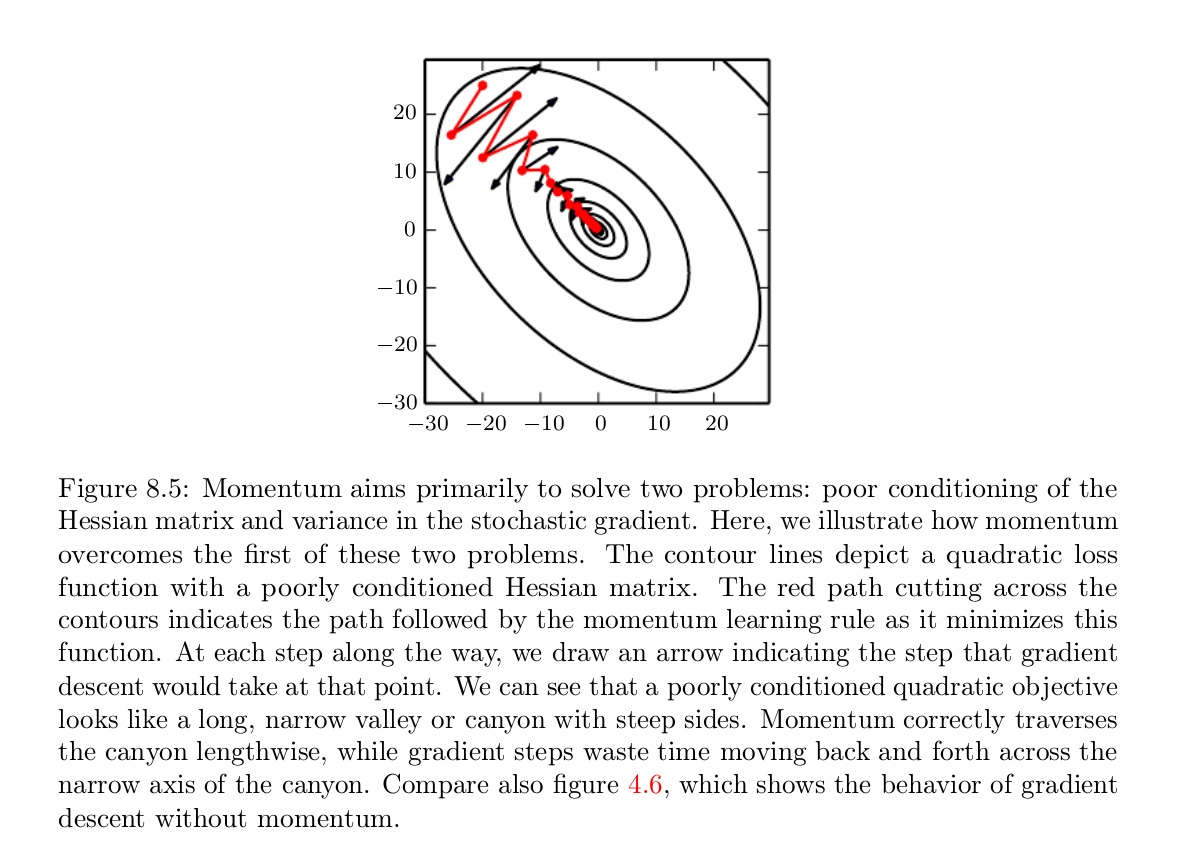
\includegraphics[width=0.8\textwidth]{figs/Momentum.png}

    {\small{Från: Deep Learning, Ian Goodfellow and Yoshua Bengio and Aaron Courville, 2016}}
\end{frame}

\begin{frame}{Startvärden}
    
    Neurala nätverk har tusentals parametrar som vi måste skatta.
    \begin{itemize}
        \item SGD är iterativt, vi börjar någonstans och ändrar dessa startvärden.
        \item Dåliga startvärden kan leda till problem.
    \end{itemize}
    Vad kan vi göra:
    \begin{itemize}
        \item Bryta symmetri mellan noderna, vikter mellan lager kan inte ha exakt samma värden.
        \item Initiera vikterna slumpmässigt
        \begin{itemize}
            \item Uniformt
            \item Normalfördelat
        \end{itemize}
        \item Bias sätts för det mesta till något värde.
        \item Att sätta startparametrar kan ses som en hyperparameter.
    \end{itemize}

\end{frame}

\begin{frame}{Adaptiv inlärningstakt}

    Kan vara svårt att få till en bra learning rate som passar alla parametrar när vi använder SGD. En idé är att anpassa learning rate för varje parameter.
    \begin{itemize}
        \item RMSProp
        \begin{itemize}
            \item Skala om gradienten beroende på träningshistorik så att vi
            \begin{itemize}
                \item tar större steg för de parametrar med små derivator.
                \item tar mindre steg för de parametrar med stora derivator.
                \item Skala med exponentiellt avtagande glidande medelvärden för tidigare gradienter.
            \end{itemize}
        \end{itemize}
        \item Adam
        \begin{itemize}
            \item Kan ses som en blandning av RMSProp och momentum.
        \end{itemize}
        \item Finns fler varianter, RMSProp och Adam är vanliga standardval för neurala nätverk och finns i de flesta paket.
        \item Finns hyperparametrar.
    \end{itemize}
    
\end{frame}

\begin{frame}{Adam och RMSProp}

    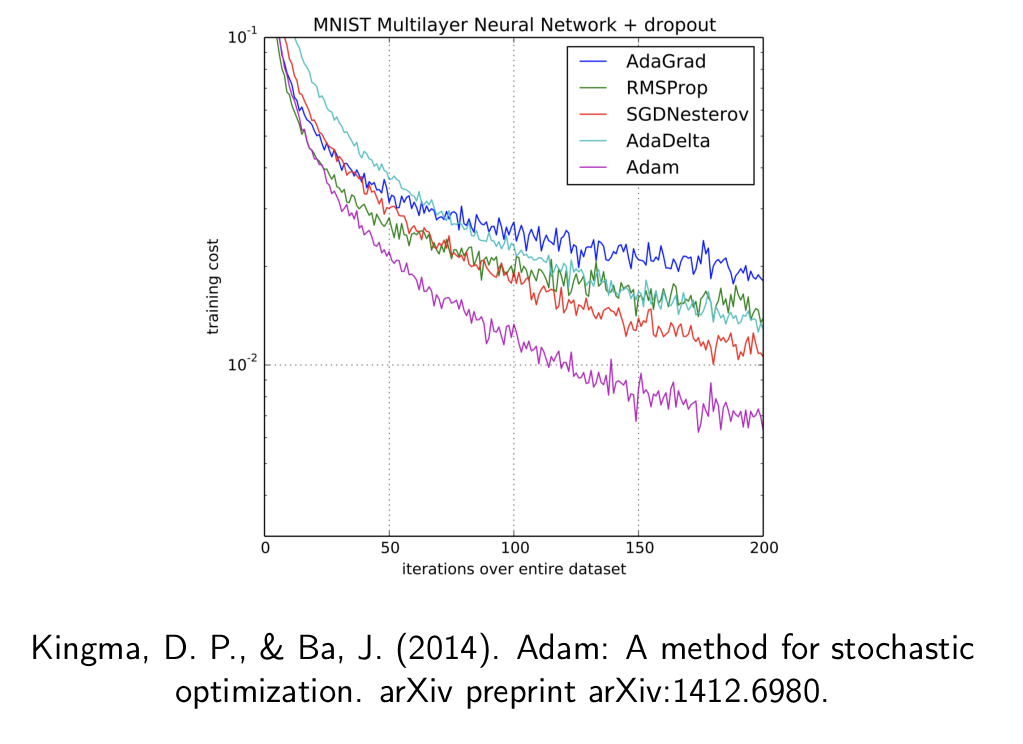
\includegraphics[width = \textwidth]{figs/DL_training_curves.png}
    
\end{frame}

\begin{frame}{Regularisering}
    Vad händer med kostandsfunktionen när vi kör Ridge/Lasso?

\end{frame}

\begin{frame}{Regularisering genom normstraff}
    
    $\text{Ridge} = \text{OLS} + \ell^2$-norm på $\beta$:
    \begin{equation*}
        \argmin_{\beta} L(\beta) = \sum_{i=1}^{n}(y_i - \hat{y})^2 + \lambda \sum_{j=1}^{p} \beta^2, \qquad \lambda \geq 0.
    \end{equation*}


    $\text{Lasso} = \text{OLS} + \ell^1$-norm på $\beta$:
    \begin{equation*}
        \argmin_{\beta} L(\beta) = \sum_{i=1}^{n}(y_i - \hat{y})^2 + \lambda \sum_{j=1}^{p} |\beta|, \qquad \lambda \geq 0.
    \end{equation*}
\end{frame}

\begin{frame}{Regularisering genom normstraff}
    
    Vi kan göra samma sak med neurala nätverk.

    Regularisering "tvingar" parametrarna att bli små (nära noll) vilket skapar en enklare funktion och minskar överanpassning.

    Vilken norm ska vi använda oss av?

\end{frame}

\begin{frame}{Regularisering genom normstraff}
    
    Generellt:
    \begin{equation*}
        \tilde{L}(\theta) = L(\theta) + \lambda \Omega(\theta),
    \end{equation*}
    \begin{description}
        \item[$L(\theta)$] kostandsfunktionen
        \item[$\Omega(\theta)$] straffterm
        \item[$\lambda$] Hyperparameter med $\lambda \geq 0$.   
    \end{description}

    Vad händer med problemet då vi ändrar $\lambda$?

\end{frame}

\begin{frame}{Neurala nätverk med normstraff}
    \begin{itemize}
        \item Använd Frobenius normen:
        \begin{equation*}
            \|\mathbf{A}\|_{F}^2 = \sum_{i=1}^{q}\sum_{j=1}^{p} a_{ij}^2 \qquad \|\mathbf{A}\|^1_{F} = \sum_{i=1}^{q}\sum_{j=1}^{p} |a_{ij}|
        \end{equation*}
        där $\mathbf{A}$ är en $p \times q$ matris.
        \item Låt $\mathbf{W}_l$ vara viktmatrisen mellan lager $l$ och $l+1$, då får vi kostnadsfunktioner
        \begin{align*}
            \tilde{L}(\theta) &= L(\theta) + \frac{\lambda}{2} \sum_{l=1}^{h} \| \mathbf{W}_l \|_{F}^{2} \\
            \tilde{L}(\theta) &= L(\theta) + \frac{\lambda}{2} \sum_{l=1}^{h} \| \mathbf{W}_l \|_{F}^{1}
        \end{align*}
    \end{itemize}
\end{frame}

\begin{frame}{Neruala nätverk med normstraff}
    \begin{itemize}
        \item Vi kan ha olika $\lambda$ för olika lager,
        \begin{equation*}
            \frac{1}{2} \sum_{l=1}^h \lambda_l \|\mathbf{W}_l\|^2_F.
        \end{equation*}
        \item Kallas ibland för weight decay (tvingar vikterna att bli mindre).
    \end{itemize}
\end{frame}

\begin{frame}{Dropout}

    \begin{itemize}
        \item I varje iteration när vi tränar vår modell med SGD:
        \begin{itemize}
            \item Låt varje nod vara noll med en viss sannolikhet.
        \end{itemize}
        \item Nätverket kan inte "lita på" några specifika kopplingar.
        \item Nätverket måste distribuera sin kapacitet över hela nätverket, motverkar överanpassning.
        \item När värdena på vikterna sprids ut över många kopplingar så blir de mindre.
        \item Dropout används vid träning, inte testning.
        \begin{itemize}
            \item Liknande effekt som vid normstraff.
        \end{itemize}
        \item Notera likheten med Random forest.
    \end{itemize}
    
\end{frame}

\begin{frame}{Dropout}
    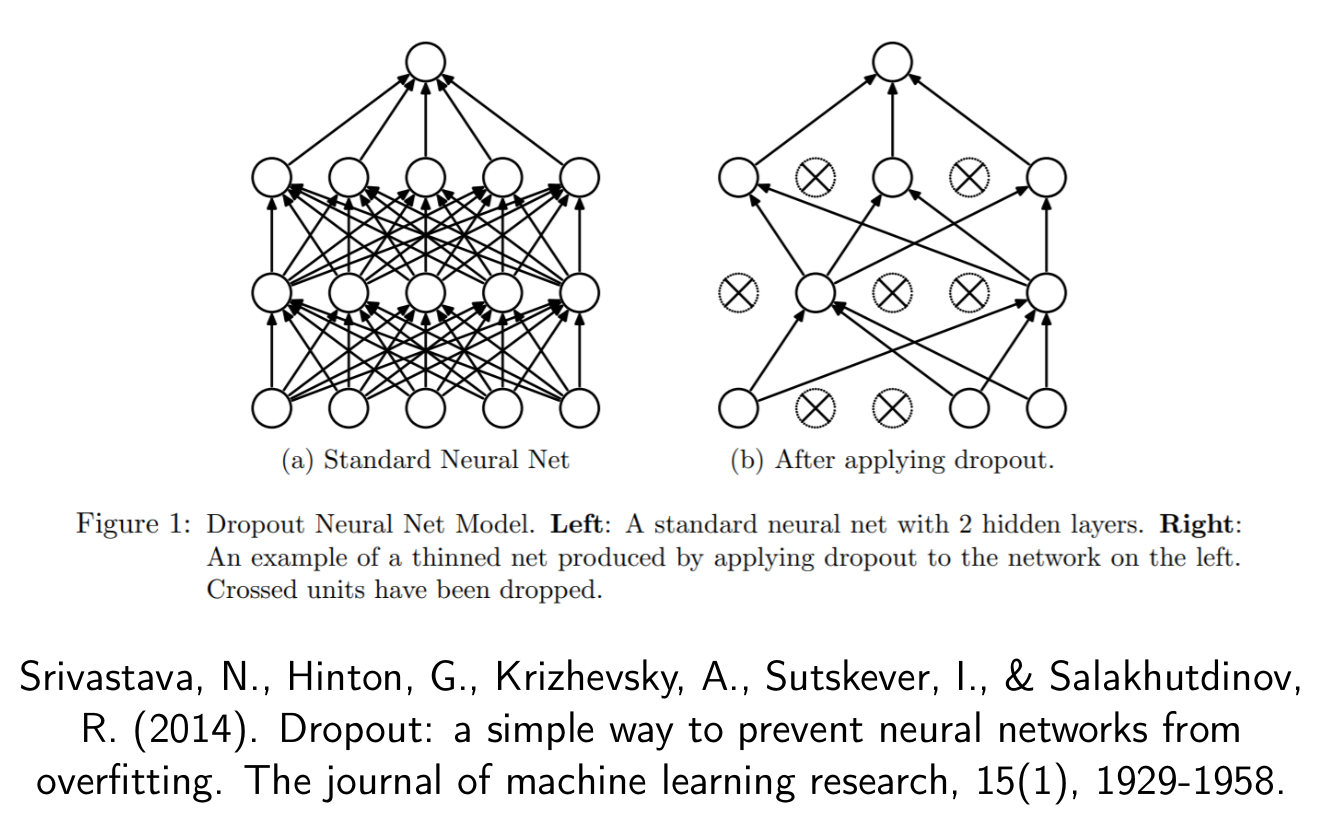
\includegraphics[width=\textwidth]{figs/dropout_example.png}
\end{frame}

\begin{frame}{Mer Regularisering}
    Det finns flera andra sätt att regularisera
    \begin{itemize}
        \item Skaffa mer träningsdata!
        \item Stoppa tidigt, använd valideringsdata för att avgöra när det är dags att stanna skattningen.
        \item Förstärk data (dataset augmentation), skapa mer artificiell data att träna på.
        \begin{itemize}
            \item Vanligt när det kommer till bilder.
            \item Spegla, rotera, beskära, addera brus m.m.
        \end{itemize}
        \item Ensamblemetoder
        \begin{itemize}
            \item Generera fler uppsättningar med startvärden och träna flera modeller: aggregera resultatet vid testdata.
        \end{itemize}
        \item Parameter Tying och Parameter Sharing
        \begin{itemize}
            \item Ha en struktur på modellen som tvingar vissa kopplingar att vara identiska eller gles m.m.
            \item T.ex. CNN, RNN
        \end{itemize}
    \end{itemize}
\end{frame}

\begin{frame}{Speciella typer av modeller}
    \begin{itemize}
        \item Residual nets: Kopplingar som hoppar över ett lager.
        \begin{itemize}
            \item Skip layer connections.
            \item Tänk: "Modellera residualerna på en linjär modell med ett neuralt nätverk".
        \end{itemize}
        \item Transfer learning:
        \begin{itemize}
            \item "Överför kunskap mellan olika problem/uppgifter".
            \item Finns olika sorter, vanlig variant: Använd förtränade nätverk på andra problem.
            \begin{itemize}
                \item Ta ett neuralt nätverk som redan är anpassat för ett problem/dataset.
                \item Starta optimering för ett annat dataset med start i de redan tränad parametrarna.
                \item Kan ses som ett avancerat sätt att välja startvärden.
                \item Ofta effektivt på mindre dataset.
            \end{itemize}
        \end{itemize}
    \end{itemize}
\end{frame}

\begin{frame}{Faltade nätverk}
    Faltade nätverk, benämns ofta CNN (Concolutional nueral networks)
    \begin{itemize}
        \item Speciella nätverk som passar för data som har en "rutnätsstruktur" (grid):
        \begin{itemize}
            \item 1-D nät: tidsserier
            \item 2-D när: bilder
            \item Tänk pixlar organiserade i en matris.
            \item \myheading{Används mycket framgångsrikt!}
            \item \href{https://dataconomy.com/2017/04/history-neural-networks/}{Lite historia}
        \end{itemize}
        \item Använder faltning mellan (minst två) lager i nätverket istället för vanliga matrismultiplikation.
    \end{itemize}
\end{frame}

\begin{frame}{Faltning}

    \begin{itemize}
        \item Faltning är en speciell typ av linjär operator.
        \item Kan defineras på lite olika sätt
        \begin{align*}
            y_t &= \int x_{\tau} h(t - \tau) \mathrm{d}\tau = \int x(t-\tau) h(\tau) \mathrm{d}\tau \\
            y(t) &= (x * h) (t)
        \end{align*}
        \item Kan ses som en sammanviktning av två kontinuerliga funktioner
        \begin{itemize}
            \item $x(t)$ är vår insignal (input).
            \item $h(t)$ är vår kärnfunktion (kernel) eller filter.
            \item $y(t)$ är vår utsignal, kan kallas feature map i DL.
        \end{itemize}
    \end{itemize}
    
\end{frame}

\begin{frame}{Faltning}

    Faltninig är en vanlig operation inom statistik, matematik, signalbehandling, reglerteknik m.m.
    \begin{itemize}
        \item Används för att filtrera signaler/tidsserier, t.ex. för att ta bort brus.
        \item Används när vi vill beräkna täthetsfunktionen för summan av två oberoende slumpvariabler.
        \begin{itemize}
            \item Givet $p(X), p(Y)$, låt $Z = X + Y$, hur beräkna $p(Z)$?
        \end{itemize}
    \end{itemize}
    
\end{frame}

\begin{frame}{Faltning}

    \begin{itemize}
        \item Om vi har diskret tid
        \begin{equation*}
            y(t) = (x * h) (t) = \sum_{\tau = - \infty}^{\infty} x(\tau) h(t - \tau),
        \end{equation*}
        $h$ blir här en vektor med värden (observera index i vektorn).
    \end{itemize}
    
\end{frame}

\begin{frame}{Faltning}

    \begin{itemize}
        \item I två dimensioner har vi
        \begin{equation*}
            y(i,j) = (x * h)(i,j) = \sum_m \sum_n x(m,n) h(i-m,j-n).
        \end{equation*}
        \item Kan generaliseras till flera dimensioner.
        \item Vi kan använda faltning som ett sätt att koppla ihop två lager i vårt neurala nätverk.
    \end{itemize}
    
\end{frame}

\begin{frame}{Varför faltning?}

    \begin{itemize}
        \item Faltning ger gles kopplingar.
        \item Spatial information: närliggande pixlar relaterar till varandra mer än pixlar långt borta.
    \end{itemize}

    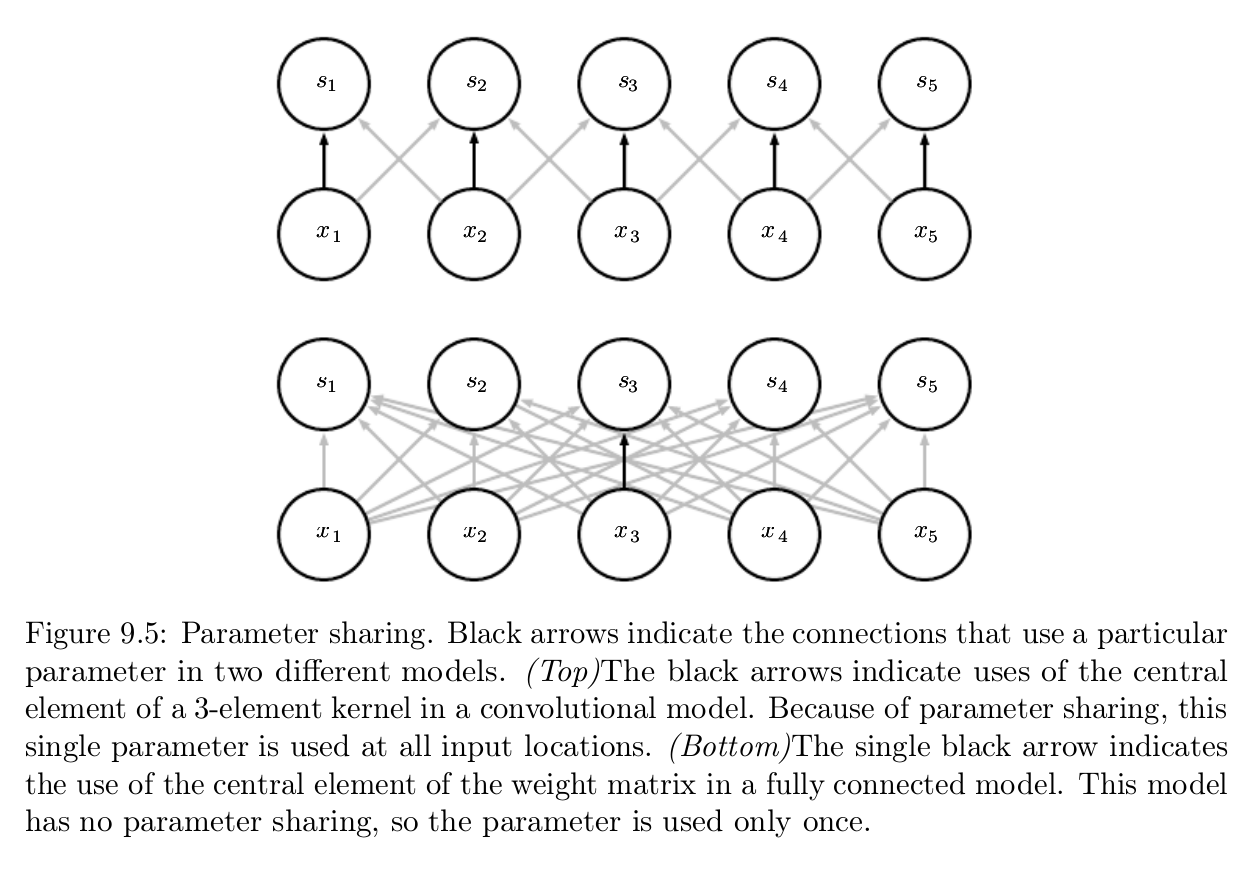
\includegraphics[width=.9\textwidth]{figs/CNN_sparse_con.png}
    
\end{frame}

\begin{frame}{Exempel: Klassificering av bilder: 2D}

    \begin{itemize}
        \item ImageNEt dataset / challenge. 1.2 miljoner bilder som träningsdata, 1000 klasser.
        \item \url{http://www.image-net.org/}
        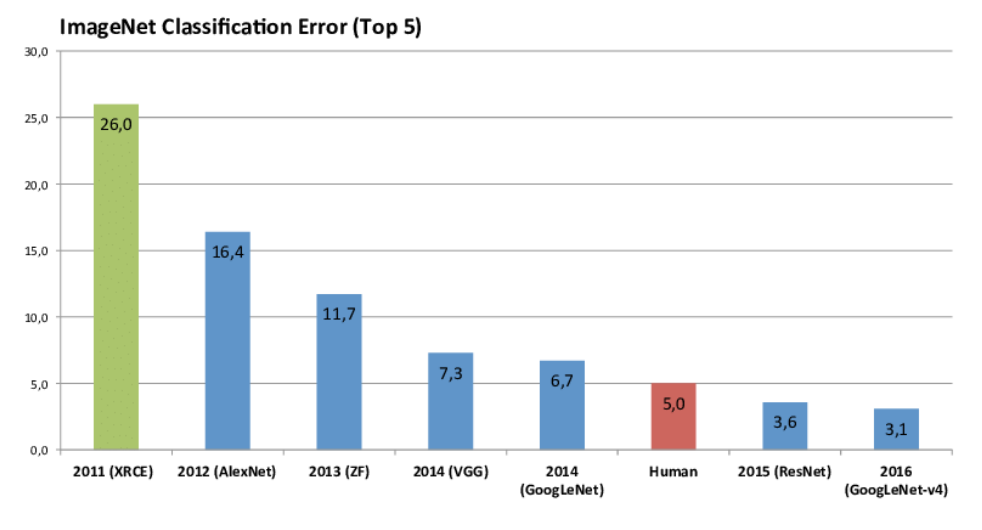
\includegraphics[width = .8\textwidth]{figs/imageNet.png}
        \item \url{https://devopedia.org/imagenet}
    \end{itemize}
    
\end{frame}

\begin{frame}{Exempel: Klassificering av bilder: 2D}

    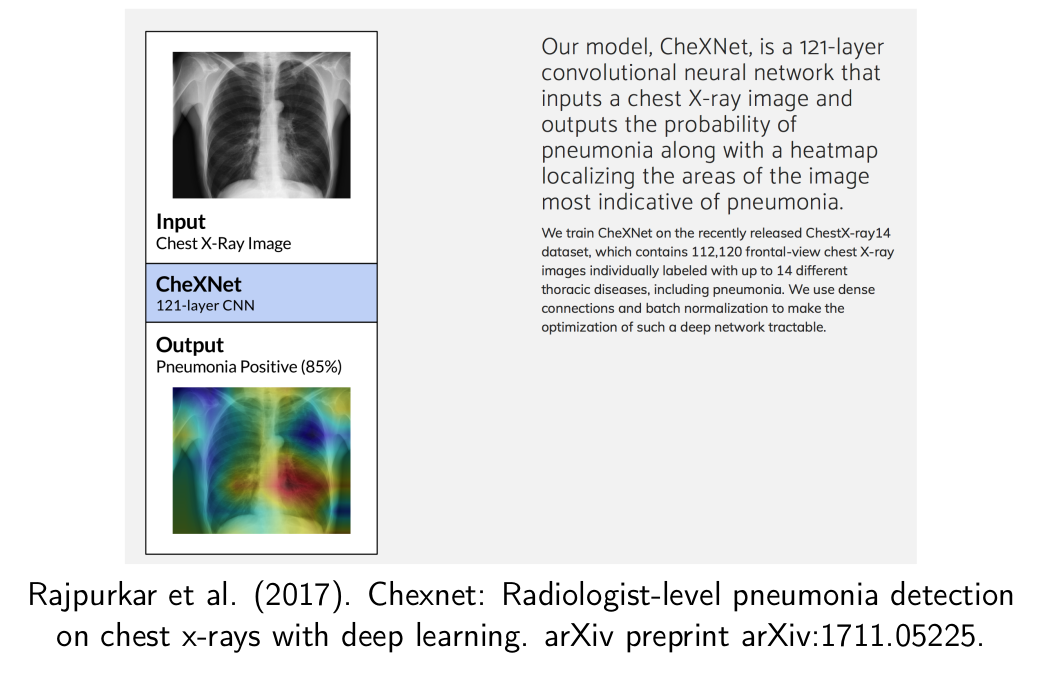
\includegraphics[width = \textwidth]{figs/Chexnet.png}
    
\end{frame}

\begin{frame}{Vad är en bild?}

    \begin{itemize}
        \item Bild: En 2D signal, varje pixel är ljusstyrka.
        \item Varje pixel har 2D koordinater $(x,y)$
        \item Varje pixel kan ha flera olika värden.
        \begin{itemize}
            \item Färgbiler, t.ex. röd grön och blå ger tre kanaler (channels).
            \item Gråskala, en kanal.
        \end{itemize}
        \item Spatial autokorrelation.
    \end{itemize}
    
\end{frame}

\begin{frame}{2D-faltning av bild}
    \href{https://ezyang.github.io/convolution-visualizer/}{Visualisering} \href{https://towardsdatascience.com/visualizing-the-fundamentals-of-convolutional-neural-networks-6021e5b07f69}{Förklaringar och räkneexempel}
    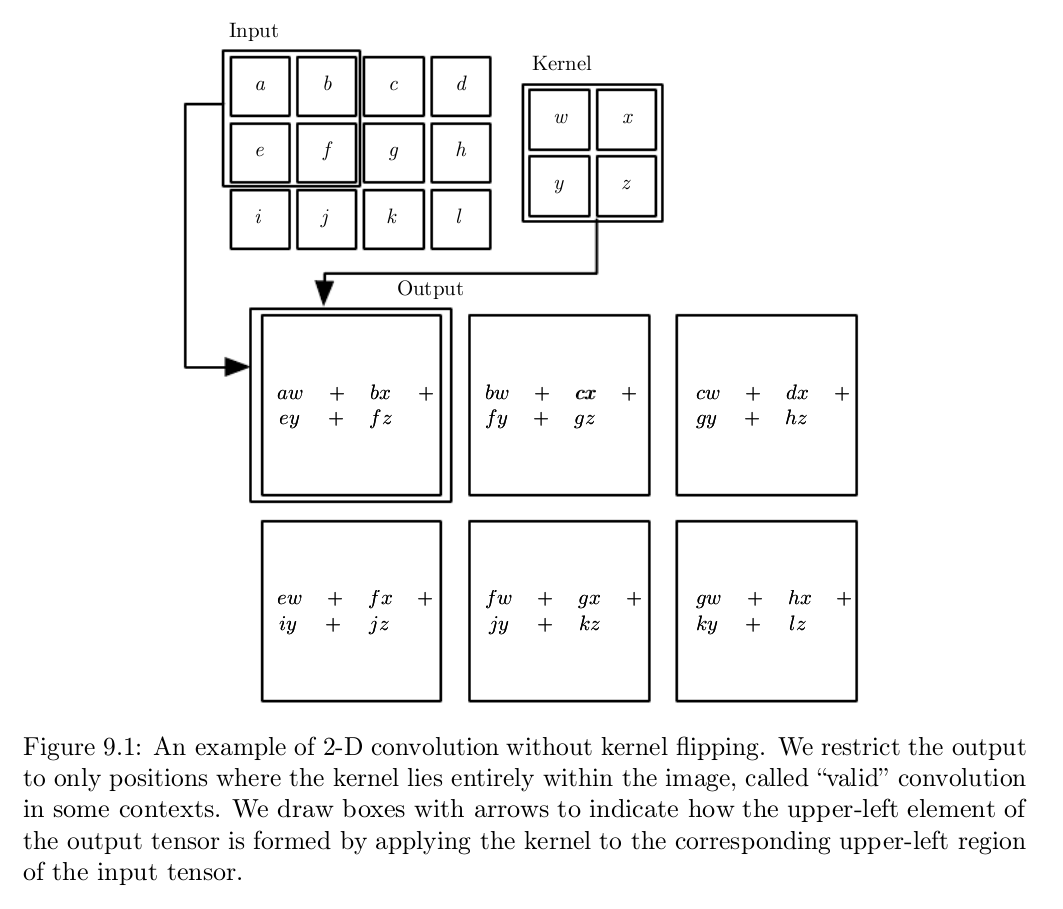
\includegraphics[width = 0.8\textwidth]{figs/2-D convolution.png}
\end{frame}

\begin{frame}{Faltade lager}
    \begin{itemize}
        \item Genomför faltning enligt föregående bild.
        \begin{itemize}
            \item Vi erhåller nu en ny matris (bild).
        \end{itemize}
        \item Aktiveringsfunktionen appliceras elementvis.
        \item Pooling:
        \begin{itemize}
            \item Tar ett rektangulärt område av bilden och beräkna sammanfattade mått.
            \item Gör resultatet från faltning invariant mot små förändringar i input data.
        \end{itemize}
        \item Notera att vi ofta vill ha fler filter per lager.
    \end{itemize}
\end{frame}

\begin{frame}{Pooling}
    
    \begin{itemize}
        \item Pooling avnänds ofta för vajre (eller vartannat) faltningslager.
        \item Hjälper till att reducera storleken på bilden.
        \begin{itemize}
            \item Betyder att senare lager inte behöver vara så stora.
        \end{itemize}
    \end{itemize}

\end{frame}

\begin{frame}{Padding och Stride}
    
    \begin{itemize}
        \item Vid faltning av bild blir resultatet mindre.
        \begin{itemize}
            \item \myheading{Padding} lägg till ett eller flera lager med 0 runt bilden.
            \item Rätt padding gör att output har samma storlek som input.
        \end{itemize}
        \item Om vi vill spara beräkningar/parametrar.
        \begin{itemize}
            \item \myheading{Stride} Hoppas över pixlar när vi glider med kernelmatrisen i faltningen.
            \item Stride = 2, hoppar över varannan pixel.
        \end{itemize}
    \end{itemize}

\end{frame}

\begin{frame}{Padding}
    
    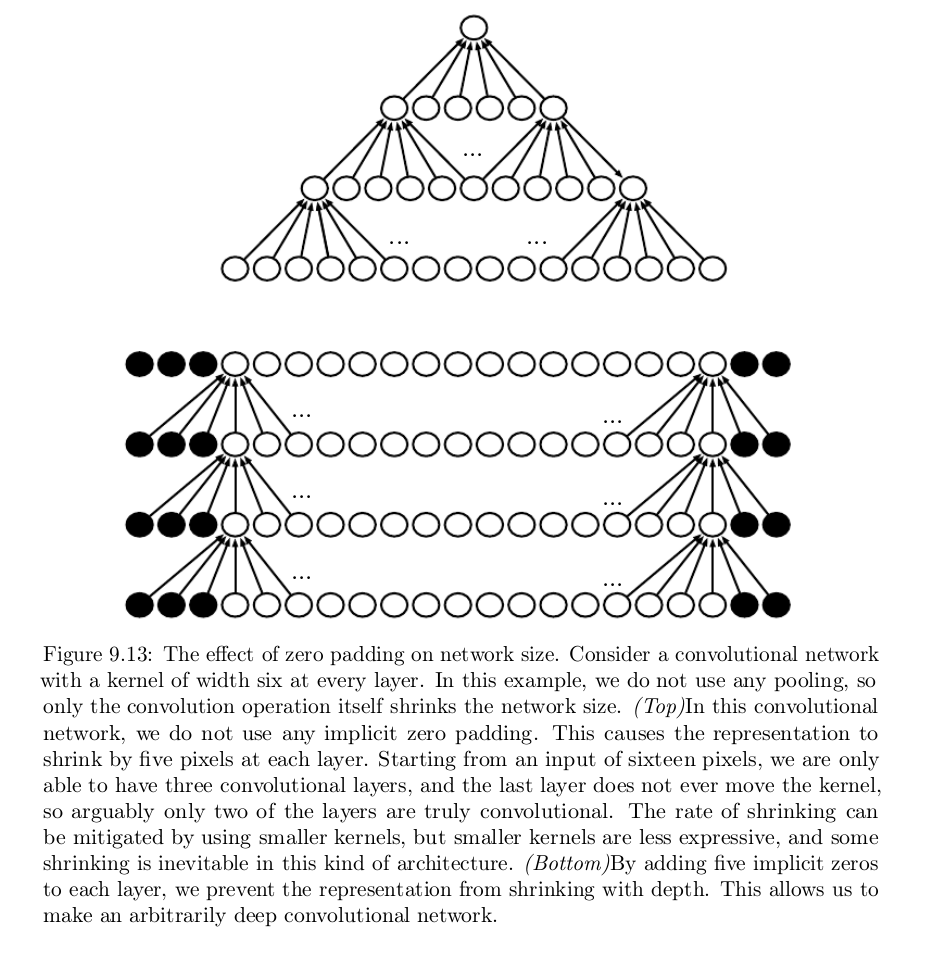
\includegraphics[height=\textheight]{figs/padding.png}

\end{frame}

\begin{frame}{Ett komplett lager}

    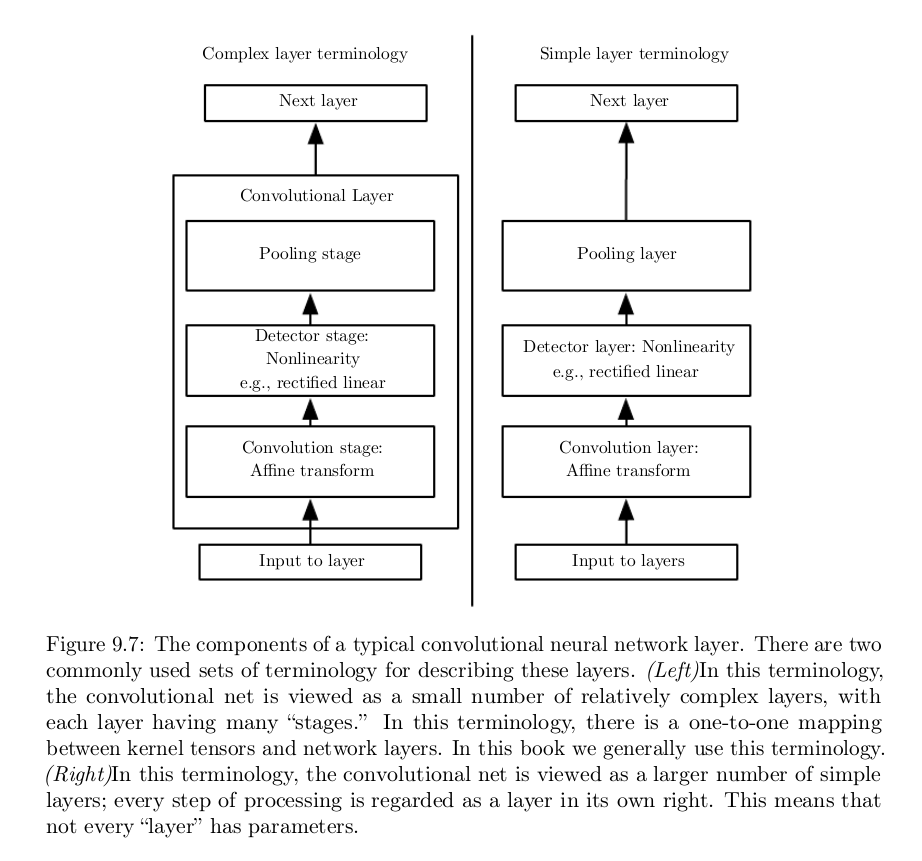
\includegraphics[height=\textheight]{figs/typical convolutional neural network layer.png}
    
\end{frame}

\begin{frame}{Sammanfattning}

    \begin{itemize}
        \item Generellt: Det är svårt att få ut bra variabler/features från bilder.
        \item Faltning är en lämplig metod!
        \begin{itemize}
            \item Relativt få parametrar.
            \item Använder lokal spatial information.
            \item Sparar beräkningar.
        \end{itemize}
        \item Vilka filter ska vi välja?
        \begin{itemize}
            \item Neurala nätverk till undsättning!
            \item Vi lär oss parametrarna i ett eller flera filter med SGD (RMSProp, Adam etc.)
        \end{itemize}
        \item Förr valdes filter "för hand" för att passa olika problem.
    \end{itemize}
    
\end{frame}

\begin{frame}{CNN Arkitektur för Klassificering}
    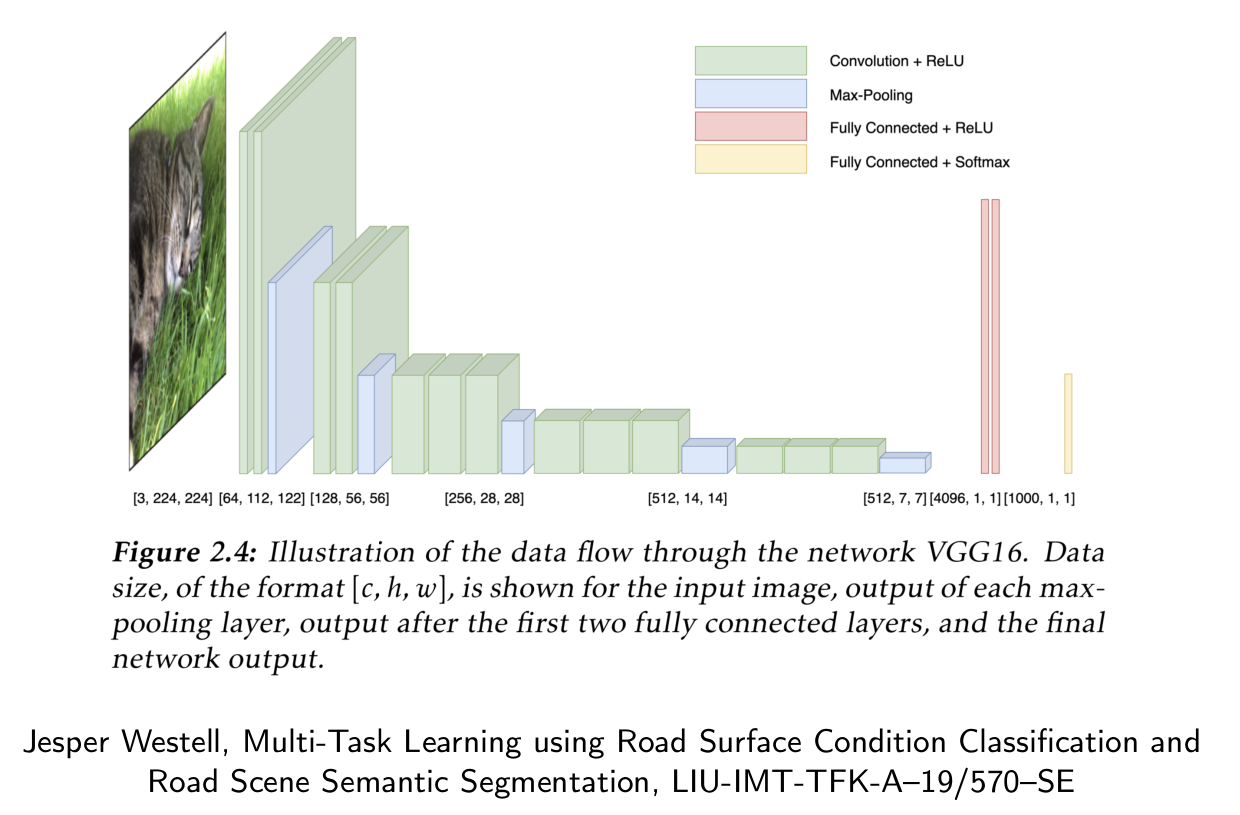
\includegraphics[width = \textwidth]{figs/CNN ARCHITECTURE.png}
\end{frame}

\end{document}